\section{HelloWorld for C}

\subsection{Scope}

In this tutorial you will build your first very simple \eTrice{} model. The goal is to learn the work flow of 
\eTrice{} and to understand a few basic features of ROOM. There are some more steps to do 
in C compared to Java. You will perform the following steps:

You will perform the following steps:

\begin{enumerate}
\item create a new model from scratch
\item add a very simple state machine to an actor
\item create a launch configuration for the C code generator
\item setup the C environment
\item generate the source code
\item run the model
\item open the message sequence chart
\end{enumerate}

Make sure that you have set up the workspace as described in \emph{Setting up the Workspace for C}.

\subsection{Create a new model from scratch}

Before you can create a new C-model, you have to create a new C project as described in \textit{Setting up 
the Workspace for C Projects}.

\begin{enumerate}
\item select the \textit{C/C++} perspective
\item select \textit{File->New->C Project} from the main menue
\item name the project \textit{HelloWorldC} 
\item the project type is \textit{Executable / Empty C Project}
\item select the Toolchain for your platform (e.g. \textit{MinGW GCC})
\end{enumerate}

Your project explorer should look like this:

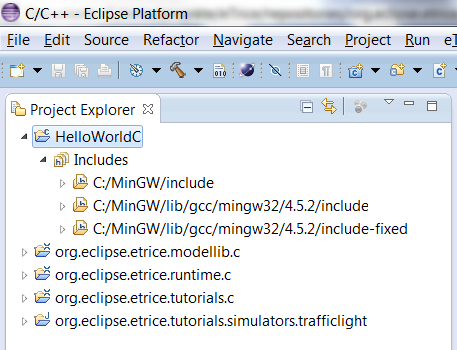
\includegraphics{images/016-HelloWorldC01.png}

The next step is to add the model folder:
Right click on the new project. Select \textit{New->Folder} and name it \textit{model}.

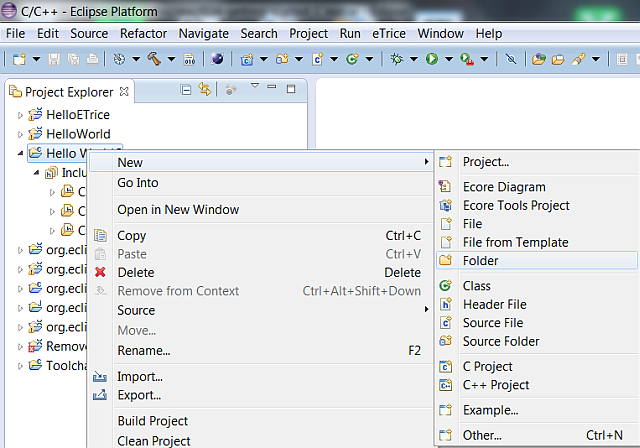
\includegraphics[width=0.8\textwidth]{images/016-HelloWorldC02.png}

Add the model file to the folder. Right click on the new folder. Select \textit{New->file} and name it 
\textit{HelloWorldC.room}.

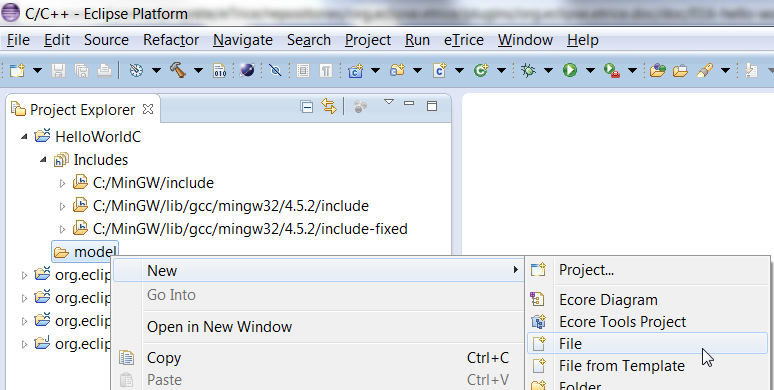
\includegraphics[width=0.8\textwidth]{images/016-HelloWorldC03.png}

Since the file extension \textit{.room} is recognized as an Xtext based format, the tool will ask you to add the Xtext nature. Answer with \textit{Yes}. 

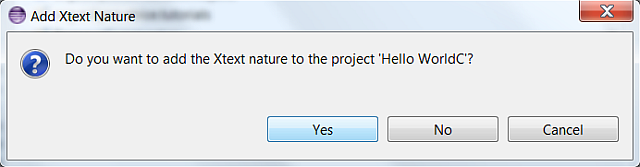
\includegraphics[width=0.8\textwidth]{images/016-HelloWorldC04.png}

Open the \emph{HelloWorld.room} file and invoke the content assist with <Ctrl>+<Space> and select \emph{RoomModel - model skeleton}.

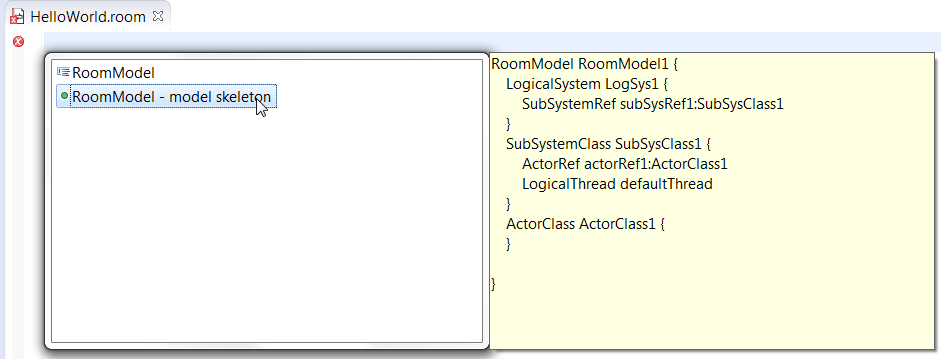
\includegraphics[width=0.8\textwidth]{images/016-HelloWorldC041.png}

Edit the template parameters by typing the new names and jumping with <Tab> from name to name.

The resulting model code should look like this:

\begin{lstlisting}[language=ROOM]
RoomModel HelloWorld_Model {

	LogicalSystem LogSys1 {
		SubSystemRef subSysRef1: SubSysClass1
	}

	SubSystemClass SubSysClass1 {
		ActorRef actorRef1: HelloWorldTop
		LogicalThread defaultThread
	}

	ActorClass HelloWorldTop { }

}
\end{lstlisting}

Now create the file model/HelloWorldC.etphys for the physical model and insert (<Ctrl>+<Space>) the code template \emph{PhysicalModel - model skeleton} without changes.

Listing for HelloWorldC.etphys :

\begin{lstlisting}[language=etPhys]
PhysicalModel PhysicalModel1 {

	PhysicalSystem PhysSys1 {
		NodeRef nodeRef1 : NodeClass1
	}

	NodeClass NodeClass1 {
		runtime = RuntimeClass1
		priomin = -10
		priomax = 10
		DefaultThread PhysicalThread1 {
			execmode = mixed
			interval = 100 ms
			prio = 0
			stacksize = 1024
			msgblocksize = 32
			msgpoolsize = 10
		}
	}

	RuntimeClass RuntimeClass1 {
		model = multiThreaded
	}
}
\end{lstlisting}

The physical model defines the setup of your nodes with their attributes like threads and mode of execution. In this case we define one node with one thread. 

The mapping model we will create now defines the mapping (deployment) of the logical elements in the .room model to the physical elements int the .etphys model. Now create the file model/HelloWorldC.etmap for the mapping model and insert (Ctrl+Space) the code template \emph{MappingModel - model skeleton} with some changes (jump with <Tab> between the template variables):

\begin{lstlisting}[language=etMap]
MappingModel MappingModel1 {
	import HelloWorld_Model.* from "HelloWorldC.room"
	import PhysicalModel1.* from "HelloWorldC.etphys"
	Mapping LogSys1 -> PhysSys1 {
		SubSystemMapping subSysRef1 -> nodeRef1 {
			ThreadMapping defaultThread -> PhysicalThread1
		}
	}
}
\end{lstlisting}

Now the workspace should look like this:

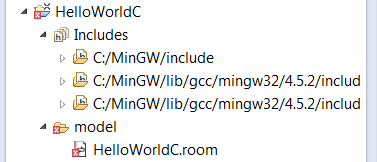
\includegraphics{images/016-HelloWorldC05.png}

The goal of \eTrice{} is to describe distributed systems on a logical level. In the current version not all 
elements will be used. But as prerequisite for further versions the following elements can be defined:
\begin{itemize}
\item the \textit{LogicalSystem} (currently optional)
\item at least one \textit{SubSystemClass} (mandatory)
\item at least one \textit{ActorClass} (mandatory)
\end{itemize}

The \textit{LogicalSystem} represents the complete distributed system and contains at least one 
\textit{SubSystemRef}. The \textit{SubSystemClass} represents an address space (e.g. a linux process or an image for a microcontroller) and contains at least one 
\textit{ActorRef}. The \textit{ActorClass} is the building block for building the hierachical structure of an application. 
A good point to start is to define a top level actor that can be used as structural root within the subsystem.

The outline view of the textual ROOM editor shows the main modeling elements in a navigation tree. You can jump to an element in the textual editor by double clicking the element in the outline view.

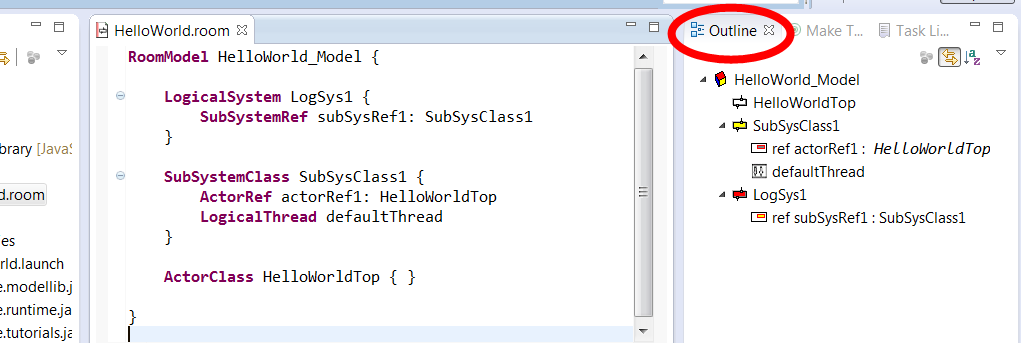
\includegraphics[width=0.8\textwidth]{images/015-HelloWorld02.png}
% !images/015-HelloWorld02.png!

\subsection{Create a state machine}

We will implement the Hello World code on the initial transition of the \textit{HelloWorldTop} actor. 
Therefore open the state machine editor by right clicking the \textit{HelloWorldTop} actor in the outline view and select \textit{Edit Behavior}.

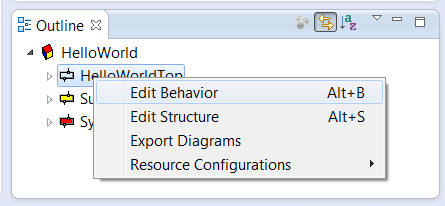
\includegraphics{images/015-HelloWorld03.png}
% !images/015-HelloWorld03.png!

The state machine editor will be opened. Drag and drop an \textit{Initial Point} from the tool box to the 
diagram into the top level state. Drag and drop a \textit{State} from the tool box to the diagram. Confirm the dialogue with \textit{ok}. Select the \textit{Transition} in the tool box and draw the transition from the \textit{Initial Point} to the State. Open the transition dialogue by double clicking the transition arrow and fill in the action code. Be aware of the different action code in Java and C.

\begin{figure}[ht]
\begin{minipage}[b]{0.45\linewidth}
	\begin{mdframed}
	\textbf{action code for Java}
	\begin{verbatim}
	System.out.println("Hello World !");
	\end{verbatim}
	\end{mdframed}
\end{minipage}
\hspace{0.5cm}
\begin{minipage}[b]{0.45\linewidth}
	\begin{mdframed}
	\textbf{action code for C}
	\begin{verbatim}
	printf("Hello World\n");
	\end{verbatim}
	\end{mdframed}
\end{minipage}
\end{figure}

 
The result should look like this:

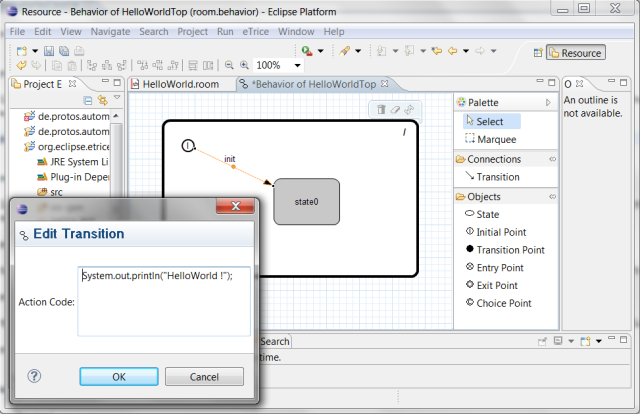
\includegraphics[width=0.8\textwidth]{images/015-HelloWorld04.png}
% !images/015-HelloWorld04.png!

Save the diagram and inspect the model (HelloWorld.room) file. Note that the textual representation was changed after saving 
the diagram.

\begin{figure}[ht]
\begin{minipage}[t]{0.50\linewidth}
\begin{mdframed}
	\textbf{room model for Java}
	\newline
\begin{lstlisting}[language=ROOM]
RoomModel HelloWorld_Model {
	LogicalSystem LogSys1 {
		SubSystemRef subSysRef1:SubSysClass1 
	}
	SubSystemClass SubSysClass1 {
		ActorRef actorRef1:HelloWorldTop 
		LogicalThread defaultThread
	}
	ActorClass HelloWorldTop {
		Structure { }
		Behavior {
			StateMachine {
				Transition init: initial -> state0 {
					action {
						"System.out.println(\"Hello World\");"
					}
				}
				State state0
			}
		}
	}
}
\end{lstlisting}
\end{mdframed}
\end{minipage}
\hspace{0.1cm}
\begin{minipage}[t]{0.50\linewidth}
\begin{mdframed}
	\textbf{room model for C}
	\newline
\begin{lstlisting}[language=ROOM]
RoomModel HelloWorld_Model {
	LogicalSystem LogSys1 {
		SubSystemRef subSysRef1: SubSysClass1
	}
	SubSystemClass SubSysClass1 {
		ActorRef actorRef1: HelloWorldTop
		LogicalThread defaultThread
	}
	ActorClass HelloWorldTop {
		Structure { }
		Behavior {
			StateMachine {
				Transition init: initial -> state0 {
					action {
						"printf(\"Hello World\\n\");"
					}
				}
				State state0
			}
		}
	}
}
\end{lstlisting}
\end{mdframed}
\end{minipage}
\end{figure}





\subsection{Create a launch configuration to start the C code generator}

Unlike in Java (where the new wizard already created a launch configuration)
a launch configuration for the C code generator must be created manually.

From the main menu \textit{Run} or the context menu \textit{Run As} in the \emph{Project Explorer} select \textit{Run Configurations} .

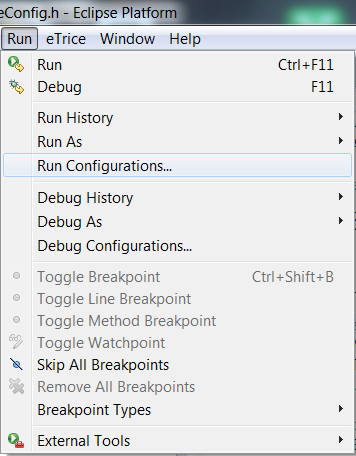
\includegraphics[width=0.8\textwidth]{images/016-HelloWorldC06.png}

Within the dialog select \textit{\eTrice{} C Generator} and click the \textit{New} button to create a new 
launch configuration.

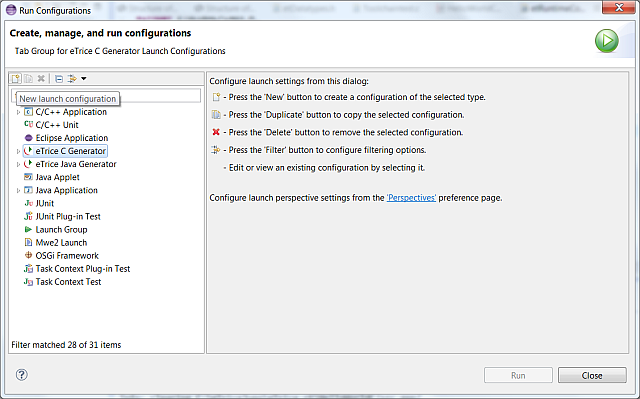
\includegraphics[width=0.8\textwidth]{images/016-HelloWorldC07.png}

A new configuration should be created. Name it \textit{gen\_HelloWorld} and add the mapping model \emph{HelloWorld.etmap} model via one of the 
\textit{add} buttons.

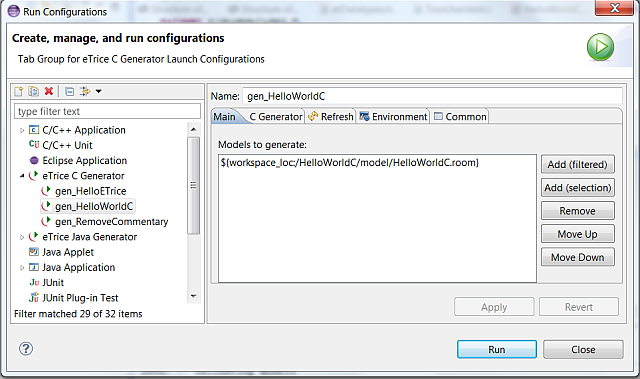
\includegraphics[width=0.8\textwidth]{images/016-HelloWorldC08.png}

The mapping model is the root model for the code generator.

To save your launch configuration, select \textit{Shared file} in the tab \textit{Common} and add the \textit{HelloWorldC} project via the 
\textit{Browse} button.

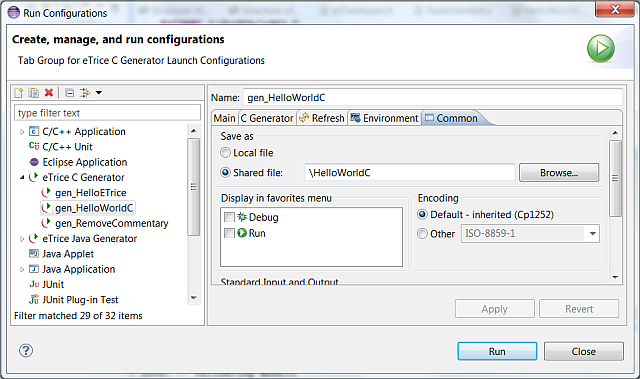
\includegraphics[width=0.8\textwidth]{images/016-HelloWorldC10.png}

Apply your changes. The new configuration should now exist in your workspace.

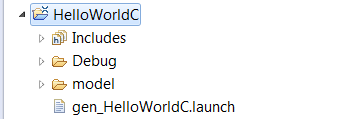
\includegraphics{images/016-HelloWorldC11.png}


\subsection{Generate the code}

Now you can generate the code. Right click on the launch configuration and run it 
as \textit{gen\_HelloWorldC}.

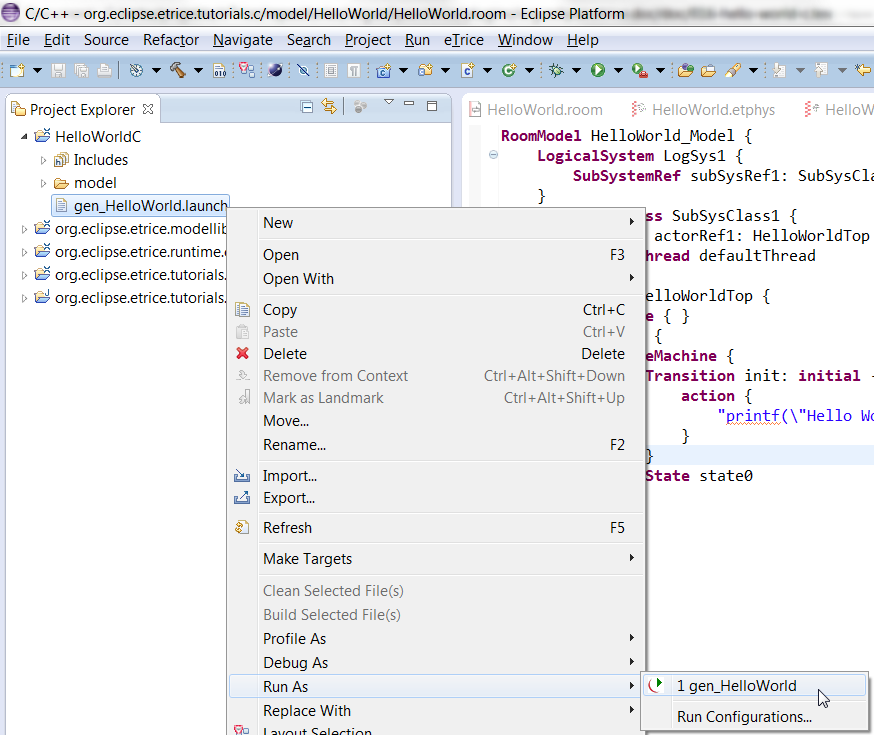
\includegraphics[width=0.8\textwidth]{images/016-HelloWorldC12.png}

The code should be generated and placed in the src-gen folder.

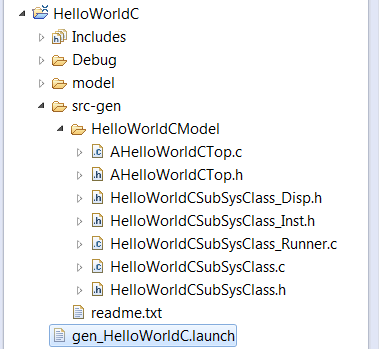
\includegraphics{images/016-HelloWorldC13.png}

\subsection{Setup the C build}

Before you can build the application you must setup the include and library paths for the runtime system. 

Right click the project and select \textit{Properties -> C/C++ Build -> Settings -> Includes}. 
Add the include path for the current project \emph{src-gen} and the runtime source folders \emph{common}, \emph{config} and the chosen platform (\emph{MT\_WIN\_MinGW} or \emph{MT\_POSIX\_GENERIC\_GCC}).

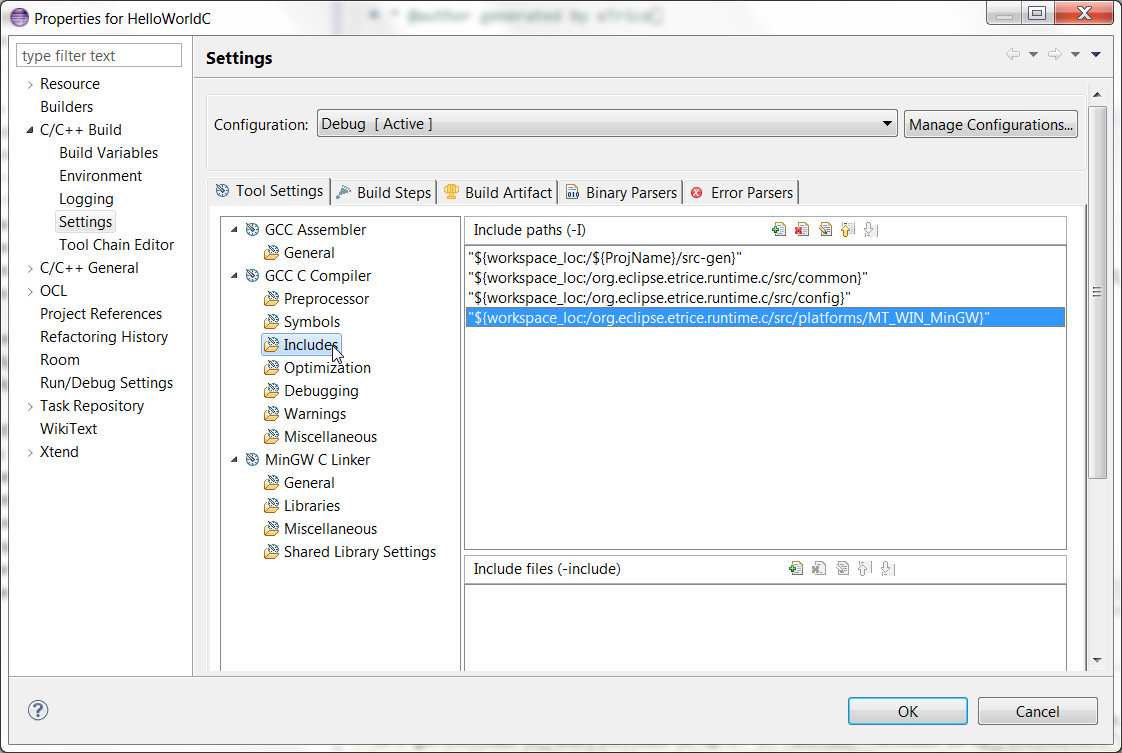
\includegraphics[width=0.8\textwidth]{images/016-HelloWorldC14.png}

Add the runtime library: \textit{Properties -> C/C++ Build -> Settings -> Libraries} and the runtime library which is appropriate for your
environment (e.g. \texttt{rt} for Linux).

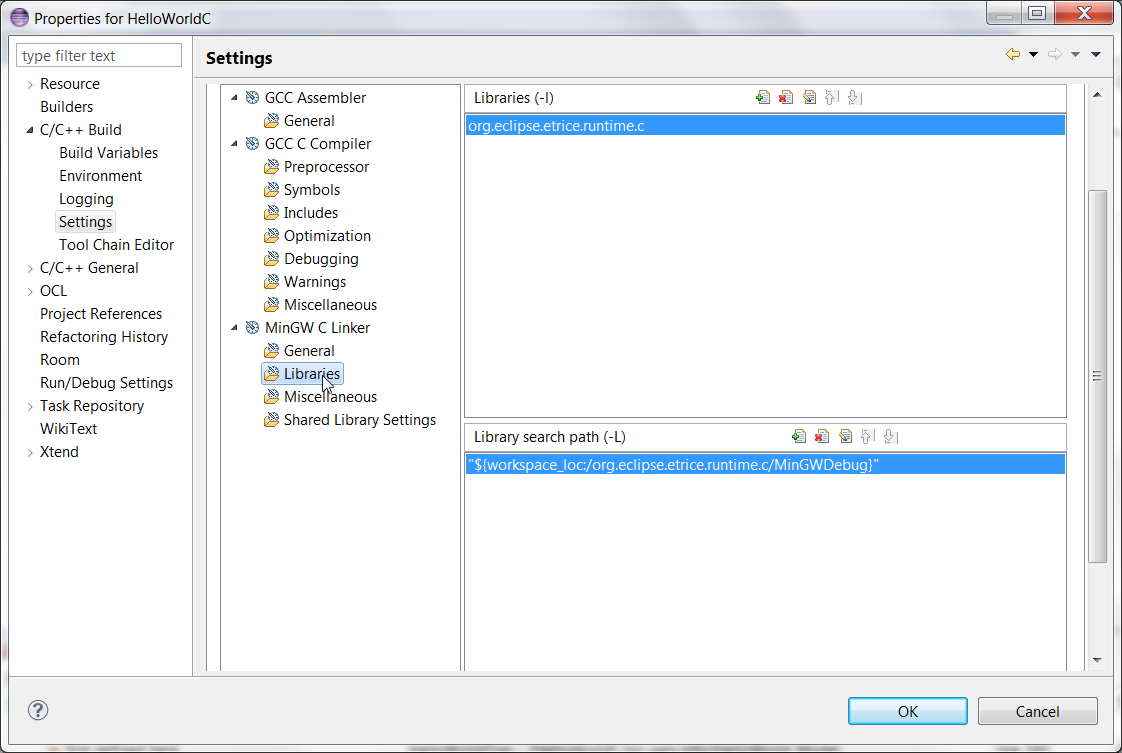
\includegraphics{images/016-HelloWorldC15.png}

The name of the library is \emph{org.eclipse.etrice.runtime.c} but the actual file name for the library is \emph{liborg.eclipse.etrice.runtime.c.a} .

\textbf{Caution:} Exclude the folder \emph{src-gen-info} from the build (this is done in the properties of this folder).
This folder is used to store temporary files for the incremental code generation and must not be compiled in order to avoid multiple definition of symbols.

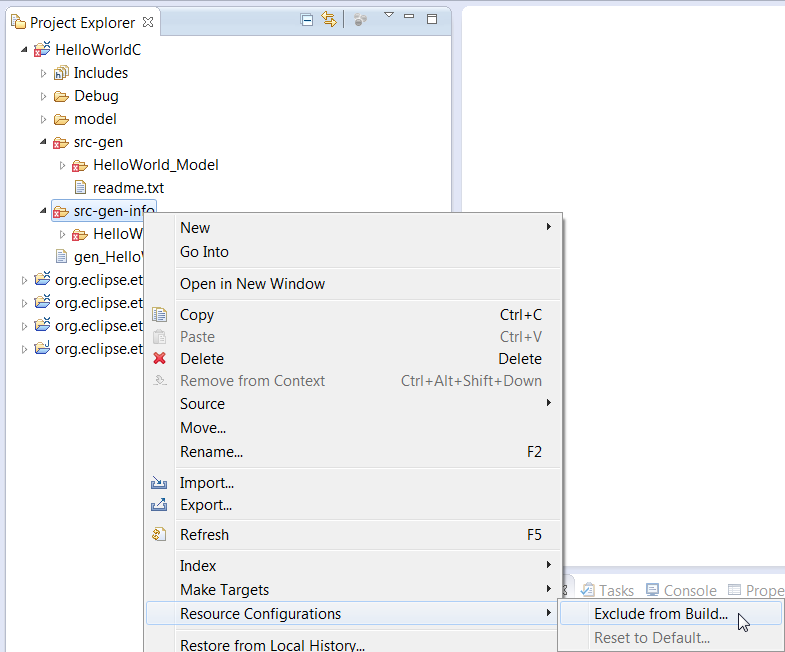
\includegraphics{images/016-HelloWorldC151.png}

\subsection{Build and run the model}

Now you can build the application. Click the build button (hammer symbol) to build the application.
Run the application in the folder \emph{Binary} as \textit{Local C/C++ Application}.
The output in the Console View should contain the message \emph{Hello World}.

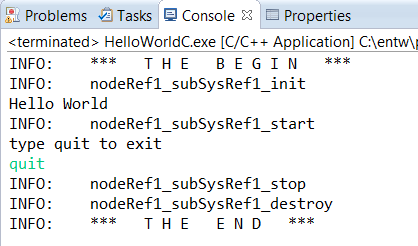
\includegraphics{images/016-HelloWorldC16.png}

\subsection{Open the Message Sequence Chart}

For debugging and learning purposes, the application produced a Message Sequence Chart and wrote it to a file. Open the file \emph{subSysRef1\_Async.seq} or \emph{msc.seq} in the folder \emph{HelloWorld/tmp/log/} using the tool Trace2UML. Create the path if not already there.

Trace2UML is an open source MSC viewer and can be obtained here:
\begin{itemize}
\item \href{http://trace2uml.tigris.org/}{Trace2UML project home and download of windows version} 
\item \href{http://apt.astade.de/}{download of the Linux package of the Astade UML tool which contains Trace2UML}
\end{itemize}
After opening the file, you should see something like this:

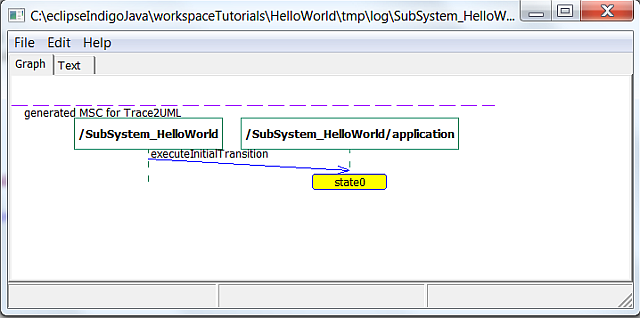
\includegraphics[width=0.6\textwidth]{images/015-HelloWorld09.png}
% !images/015-HelloWorld09.png!

The Actor with the instance path \emph{/LogSys1/subSysRef1/actorRef1} is in the state \emph{state0}. 
This is the simplest possible MSC. The MSCs for further tutorials will contain more information.


\subsection{Summary}

You are now familiar with all necessary steps to create, build and run an \eTrice{} C model from scratch. You 
are able to create a launch configuration to start the code generator and to perform all necessary 
settings to compile and link the application.  

The next tutorial provides an exercise to get more familiar with these working steps.
